\documentclass{standalone}
\usepackage{tikz}
\usetikzlibrary{patterns, positioning}


\begin{document}
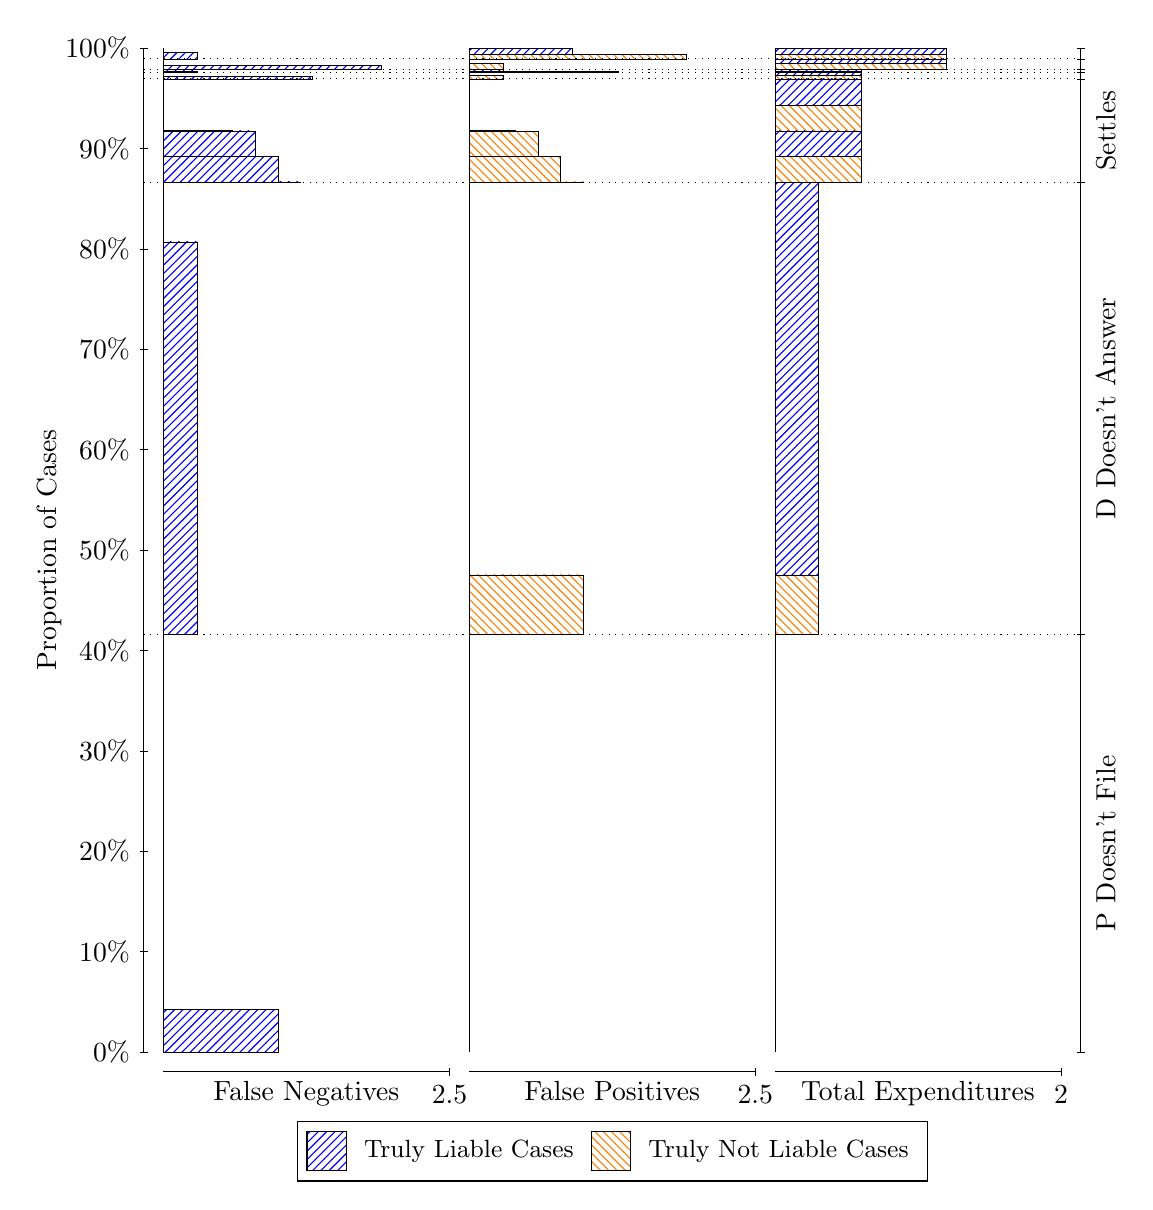
\begin{tikzpicture}
\draw[black, very thin] (1.5,1.75) -- (1.5,14.5);
\node[rotate=90, text=black, anchor=center] at (0.3, 8.125) {Proportion of Cases};
\draw[black, very thin] (1.45,1.75) -- (1.55,1.75);
\node[text=black, anchor=east] at (1.45, 1.75) {0\%};
\draw[black, very thin] (1.45,3.025) -- (1.55,3.025);
\node[text=black, anchor=east] at (1.45, 3.025) {10\%};
\draw[black, very thin] (1.45,4.3) -- (1.55,4.3);
\node[text=black, anchor=east] at (1.45, 4.3) {20\%};
\draw[black, very thin] (1.45,5.575) -- (1.55,5.575);
\node[text=black, anchor=east] at (1.45, 5.575) {30\%};
\draw[black, very thin] (1.45,6.85) -- (1.55,6.85);
\node[text=black, anchor=east] at (1.45, 6.85) {40\%};
\draw[black, very thin] (1.45,8.125) -- (1.55,8.125);
\node[text=black, anchor=east] at (1.45, 8.125) {50\%};
\draw[black, very thin] (1.45,9.4) -- (1.55,9.4);
\node[text=black, anchor=east] at (1.45, 9.4) {60\%};
\draw[black, very thin] (1.45,10.675) -- (1.55,10.675);
\node[text=black, anchor=east] at (1.45, 10.675) {70\%};
\draw[black, very thin] (1.45,11.95) -- (1.55,11.95);
\node[text=black, anchor=east] at (1.45, 11.95) {80\%};
\draw[black, very thin] (1.45,13.225) -- (1.55,13.225);
\node[text=black, anchor=east] at (1.45, 13.225) {90\%};
\draw[black, very thin] (1.45,14.5) -- (1.55,14.5);
\node[text=black, anchor=east] at (1.45, 14.5) {100\%};

\draw[black, very thin] (13.4,1.75) -- (13.4,14.5);
\draw[black, very thin] (13.35,1.75) -- (13.45,1.75);
\node[anchor=west] at (13.35, 1.75) {};
\draw[black, very thin] (13.35,7.0516) -- (13.45,7.0516);
\node[anchor=west] at (13.35, 7.0516) {};
\draw[black, very thin] (13.35,12.796) -- (13.45,12.796);
\node[anchor=west] at (13.35, 12.796) {};
\draw[black, very thin] (13.35,14.109) -- (13.45,14.109);
\node[anchor=west] at (13.35, 14.109) {};
\draw[black, very thin] (13.35,14.186) -- (13.45,14.186);
\node[anchor=west] at (13.35, 14.186) {};
\draw[black, very thin] (13.35,14.225) -- (13.45,14.225);
\node[anchor=west] at (13.35, 14.225) {};
\draw[black, very thin] (13.35,14.362) -- (13.45,14.362);
\node[anchor=west] at (13.35, 14.362) {};
\draw[black, very thin] (13.35,14.5) -- (13.45,14.5);
\node[anchor=west] at (13.35, 14.5) {};

\draw[black, very thin, pattern color=blue, pattern=north east lines] (1.75,1.75) rectangle (3.2033,2.2912);
\draw[black, very thin, pattern color=orange, pattern=north west lines] (1.75,2.2912) rectangle (1.75,7.0516);
\draw[black, very thin, pattern color=blue, pattern=north east lines] (1.75,7.0516) rectangle (2.186,12.037);
\draw[black, very thin, pattern color=orange, pattern=north west lines] (1.75,12.037) rectangle (1.75,12.796);
\draw[black, very thin, pattern color=blue, pattern=north east lines] (1.75,12.796) rectangle (3.494,12.801);
\draw[black, very thin, pattern color=blue, pattern=north east lines] (1.75,12.801) rectangle (3.2033,13.124);
\draw[black, very thin, pattern color=blue, pattern=north east lines] (1.75,13.124) rectangle (3.058,13.125);
\draw[black, very thin, pattern color=blue, pattern=north east lines] (1.75,13.125) rectangle (2.9127,13.448);
\draw[black, very thin, pattern color=blue, pattern=north east lines] (1.75,13.448) rectangle (2.622,13.451);
\draw[black, very thin, pattern color=orange, pattern=north west lines] (1.75,13.451) rectangle (1.75,14.109);
\draw[black, very thin, pattern color=blue, pattern=north east lines] (1.75,14.109) rectangle (3.6393,14.141);
\draw[black, very thin, pattern color=orange, pattern=north west lines] (1.75,14.141) rectangle (1.75,14.186);
\draw[black, very thin, pattern color=blue, pattern=north east lines] (1.75,14.186) rectangle (2.186,14.209);
\draw[black, very thin, pattern color=orange, pattern=north west lines] (1.75,14.209) rectangle (1.75,14.225);
\draw[black, very thin, pattern color=blue, pattern=north east lines] (1.75,14.225) rectangle (4.5113,14.283);
\draw[black, very thin, pattern color=orange, pattern=north west lines] (1.75,14.283) rectangle (1.75,14.362);
\draw[black, very thin, pattern color=blue, pattern=north east lines] (1.75,14.362) rectangle (2.186,14.442);
\draw[black, very thin, pattern color=orange, pattern=north west lines] (1.75,14.442) rectangle (1.75,14.5);
\draw[black, very thin, pattern color=orange, pattern=north west lines] (5.6333,1.75) rectangle (5.6333,6.5104);
\draw[black, very thin, pattern color=blue, pattern=north east lines] (5.6333,6.5104) rectangle (5.6333,7.0516);
\draw[black, very thin, pattern color=orange, pattern=north west lines] (5.6333,7.0516) rectangle (7.0867,7.8102);
\draw[black, very thin, pattern color=blue, pattern=north east lines] (5.6333,7.8102) rectangle (5.6333,12.796);
\draw[black, very thin, pattern color=orange, pattern=north west lines] (5.6333,12.796) rectangle (7.0867,12.799);
\draw[black, very thin, pattern color=orange, pattern=north west lines] (5.6333,12.799) rectangle (6.796,13.122);
\draw[black, very thin, pattern color=orange, pattern=north west lines] (5.6333,13.122) rectangle (6.6507,13.123);
\draw[black, very thin, pattern color=orange, pattern=north west lines] (5.6333,13.123) rectangle (6.5053,13.446);
\draw[black, very thin, pattern color=orange, pattern=north west lines] (5.6333,13.446) rectangle (6.2147,13.453);
\draw[black, very thin, pattern color=blue, pattern=north east lines] (5.6333,13.453) rectangle (5.6333,14.109);
\draw[black, very thin, pattern color=orange, pattern=north west lines] (5.6333,14.109) rectangle (6.0693,14.154);
\draw[black, very thin, pattern color=blue, pattern=north east lines] (5.6333,14.154) rectangle (5.6333,14.186);
\draw[black, very thin, pattern color=orange, pattern=north west lines] (5.6333,14.186) rectangle (7.5227,14.202);
\draw[black, very thin, pattern color=blue, pattern=north east lines] (5.6333,14.202) rectangle (6.0693,14.225);
\draw[black, very thin, pattern color=orange, pattern=north west lines] (5.6333,14.225) rectangle (6.0693,14.305);
\draw[black, very thin, pattern color=blue, pattern=north east lines] (5.6333,14.305) rectangle (5.6333,14.362);
\draw[black, very thin, pattern color=orange, pattern=north west lines] (5.6333,14.362) rectangle (8.3947,14.42);
\draw[black, very thin, pattern color=blue, pattern=north east lines] (5.6333,14.42) rectangle (6.9413,14.5);
\draw[black, very thin, pattern color=orange, pattern=north west lines] (9.5167,1.75) rectangle (9.5167,6.5104);
\draw[black, very thin, pattern color=blue, pattern=north east lines] (9.5167,6.5104) rectangle (9.5167,7.0516);
\draw[black, very thin, pattern color=orange, pattern=north west lines] (9.5167,7.0516) rectangle (10.062,7.8102);
\draw[black, very thin, pattern color=blue, pattern=north east lines] (9.5167,7.8102) rectangle (10.062,12.796);
\draw[black, very thin, pattern color=orange, pattern=north west lines] (9.5167,12.796) rectangle (10.607,13.122);
\draw[black, very thin, pattern color=blue, pattern=north east lines] (9.5167,13.122) rectangle (10.607,13.449);
\draw[black, very thin, pattern color=orange, pattern=north west lines] (9.5167,13.449) rectangle (10.607,13.779);
\draw[black, very thin, pattern color=blue, pattern=north east lines] (9.5167,13.779) rectangle (10.607,14.109);
\draw[black, very thin, pattern color=orange, pattern=north west lines] (9.5167,14.109) rectangle (10.607,14.154);
\draw[black, very thin, pattern color=blue, pattern=north east lines] (9.5167,14.154) rectangle (10.607,14.186);
\draw[black, very thin, pattern color=orange, pattern=north west lines] (9.5167,14.186) rectangle (10.607,14.202);
\draw[black, very thin, pattern color=blue, pattern=north east lines] (9.5167,14.202) rectangle (10.607,14.225);
\draw[black, very thin, pattern color=orange, pattern=north west lines] (9.5167,14.225) rectangle (11.697,14.305);
\draw[black, very thin, pattern color=blue, pattern=north east lines] (9.5167,14.305) rectangle (11.697,14.362);
\draw[black, very thin, pattern color=orange, pattern=north west lines] (9.5167,14.362) rectangle (11.697,14.42);
\draw[black, very thin, pattern color=blue, pattern=north east lines] (9.5167,14.42) rectangle (11.697,14.5);
\draw[black, dotted] (1.5,7.0516) -- (13.4,7.0516);
\draw[black, dotted] (1.5,12.796) -- (13.4,12.796);
\draw[black, dotted] (1.5,14.109) -- (13.4,14.109);
\draw[black, dotted] (1.5,14.186) -- (13.4,14.186);
\draw[black, dotted] (1.5,14.225) -- (13.4,14.225);
\draw[black, dotted] (1.5,14.362) -- (13.4,14.362);
\draw[black, very thin] (1.75,1.5) -- (5.3833,1.5);
\node[text=black, anchor=north] at (3.5667, 1.5) {False Negatives};
\draw[black, very thin] (5.3833,1.45) -- (5.3833,1.55);
\node[text=black, anchor=north] at (5.3833, 1.45) {2.5};

\draw[black, very thin] (5.6333,1.5) -- (9.2667,1.5);
\node[text=black, anchor=north] at (7.45, 1.5) {False Positives};
\draw[black, very thin] (9.2667,1.45) -- (9.2667,1.55);
\node[text=black, anchor=north] at (9.2667, 1.45) {2.5};

\draw[black, very thin] (9.5167,1.5) -- (13.15,1.5);
\node[text=black, anchor=north] at (11.333, 1.5) {Total Expenditures};
\draw[black, very thin] (13.15,1.45) -- (13.15,1.55);
\node[text=black, anchor=north] at (13.15, 1.45) {2};

\node[text=black, centered, rotate=90] at (13.72, 4.4008) {P Doesn't File};
\node[text=black, centered, rotate=90] at (13.72, 9.9236) {D Doesn't Answer};
\node[text=black, centered, rotate=90] at (13.72, 13.452) {Settles};





\draw (7.449999999999999,1.5) node[draw=none] (baseCoordinate) {};
\begin{scope}[align=center]
        \matrix[scale=0.5, draw=black, below=0.5cm of baseCoordinate, nodes={draw}, column sep=0.1cm]{
            \node[rectangle, draw, minimum width=0.5cm, minimum height=0.5cm, pattern color=blue, pattern=north east lines] {}; &
            \node[draw=none, font=\small, text=black] (B) {Truly Liable Cases}; &
            \node[rectangle, draw, minimum width=0.5cm, minimum height=0.5cm, pattern color=orange, pattern=north west lines] {}; &
            \node[draw=none, font=\small, text=black] (B) {Truly Not Liable Cases}; \\
            };
\end{scope}

\end{tikzpicture}
\end{document}